\section{Evaluation}
\label{sec:experiment}
\label{sec:results}

We evaluate the abstraction twice, and report negative results alongside
positive ones:

\begin{itemize}
    \item \textbf{RQ1 (as an analysis).} How accurately does $\phi$ label
          operations, per class, and what does component-based recognition of
          wrapped APIs buy and cost relative to exact allow-listing?
    \item \textbf{RQ2 (as a representation).} With graph, backbone and
          training budget held fixed, how much does replacing lexical node
          features with the abstraction change cross-project detection?
    \item \textbf{RQ3 (generality).} Does the effect hold across corpora and
          across message-passing schemes?
    \item \textbf{RQ4 (granularity).} Does a finer operation alphabet recover
          signal that the coarsest one discards?
\end{itemize}

\subsection{Setup}

\subsubsection{Corpora}
We use BigVul~\cite{fan2020bigvul}, DiverseVul~\cite{chen2023diversevul} and
Devign~\cite{zhou2019devign}, loaded from pinned public mirrors. Each is
sampled to 8{,}000 functions. We disclose two properties that are usually left
implicit and that materially affect cross-project claims: the sample is taken
in corpus order rather than at random, and project mass is highly
concentrated --- in BigVul, Chrome and \texttt{linux} together supply about
two thirds of the functions.

% Generated by experiments/emit_tables.py -- DO NOT EDIT BY HAND.
% Every value is read from experiments/results/*.json.

\begin{table}[t]
\centering
\caption{Corpus properties measured on our samples. Project concentration is
reported because it determines whether a nominally cross-project split is
meaningful: in BigVul the two largest repositories supply two thirds of the
functions, which is why they are held train-only
(Section~\ref{sec:protocol}). Generated mechanically from result files.}
\label{tab:corpora}
\begin{tabular}{lrrrrr}
\toprule
Corpus & Functions & Prevalence & Projects & Top-2 share & Nodes/Edges \\
\midrule
BigVul & 8,000 & 0.054 & 134 & 66.3\% & 90 / 231 \\
DiverseVul & 8,000 & 0.055 & 580 & 27.4\% & 77 / 195 \\
Devign & 8,000 & 0.473 & 2 & 100.0\% & 134 / 351 \\
\bottomrule
\end{tabular}
\end{table}


Table~\ref{tab:corpora} records these properties. Devign is included for the
analysis validation of Section~\ref{sec:rq_analysis} but \emph{excluded from
all cross-project claims}: with two repositories, a project-disjoint split
degenerates to training on one and testing on the other, and any federated or
heterogeneity framing over it would be describing a single codebase.

\subsubsection{What the abstraction retains and discards}
Table~\ref{tab:node_dist} gives the node-type distribution under
$\phi_8$ on BigVul. Three quarters of AST nodes carry no operation semantics
and are labelled $\bot$; they still contribute their grammar kind through
Eq.~\eqref{eq:features}, so they are not featureless. The distribution also
explains a negative result in advance: the memory-operation class that
motivates the taxonomy accounts for $0.43\%$ of nodes, so subdividing it
(Section~\ref{sec:rq_negative}) cannot move an aggregate metric however
semantically justified the distinction is.

% Generated by experiments/emit_tables.py -- DO NOT EDIT BY HAND.
% Every value is read from experiments/results/*.json.

\begin{table}[t]
\centering
\caption{Node-type distribution under $\phi_8$ (BigVul). $\bot$
(\texttt{UNKNOWN}) nodes carry no operation label but retain their grammar
kind. Generated mechanically from result files.}
\label{tab:node_dist}
\begin{tabular}{lr@{\hskip 2em}lr}
\toprule
Type & Share & Type & Share \\
\midrule
$\bot$ (\texttt{UNKNOWN}) & 75.73\% & \texttt{COMPARISON} & 2.64\% \\
\texttt{PTR\_DEREF} & 6.46\% & \texttt{ARITH\_OP} & 1.59\% \\
\texttt{CALL\_SITE} & 5.31\% & \texttt{ARRAY\_INDEX} & 0.49\% \\
\texttt{CONTROL\_BRANCH} & 3.97\% & \texttt{MEMORY\_ACCESS} & 0.43\% \\
\texttt{ASSIGN} & 3.38\% & & \\
\bottomrule
\end{tabular}
\end{table}


\subsubsection{Deduplication}
Near-duplicate functions are removed \emph{before} any split. Vendored code
appears under several project names, so without this step a held-out function
can have a twin in training and project-disjointness is defeated silently.
Signatures are computed over the abstracted node sequence, which catches
renamed copies that text hashing misses; 2--3\% of functions are removed.

\subsubsection{Cross-project protocol}
\label{sec:protocol}
Evaluation is repeated project-level GroupKFold: projects are dealt into five
folds, no project is split, and each fold is used once as the test set. Two
provisions matter. First, projects too large to be placed without dominating a
fold --- Chrome and \texttt{linux} --- are held \emph{train-only} and reported
as such, so that no fold labelled ``cross-project'' is in fact an evaluation
on one repository. Second, all vocabularies and label bucketings are fitted on
training projects only.

Per-corpus fold statistics differ according to project distributions. In BigVul,
the resulting folds are stable: test fraction $0.071$ on every fold, 39--49 test
projects per fold. In DiverseVul, folds contain 1{,}223--1{,}224 test functions across
115--116 projects, yielding a test fraction near $0.16$.

We disclose that even with Chrome and \texttt{linux} held train-only, project size
concentration remains visible among held-out projects: in BigVul folds 0 and 5,
the \texttt{Android} repository accounts for $69\%$ of test set samples. Furthermore,
across repeated GroupKFold split assignments, repeat folds share a small subset of test
projects (e.g., 8 of 39 projects overlap between repeat folds 0 and 5).

We report AUC as the primary metric and AUPRC as the imbalanced-data
companion, both threshold-free. F1 is reported only against an explicit floor:
the trivial classifier that labels every function vulnerable achieves
$F_1 = 0.161$ at the $8.8\%$ prevalence of these test sets, which is above
several F1 values reported as results in the literature.

\subsubsection{Statistical treatment}
Fold-level means are reported with standard deviations, but inference uses a
\emph{cluster bootstrap} that resamples held-out projects with replacement,
because functions within a repository share style, APIs and often
near-duplicate code and are therefore not independent. We report the paired
difference between systems with a 95\% percentile interval and a two-sided
bootstrap $p$-value. Where an interval crosses zero we say so and draw no
conclusion.

Two details of this procedure are declared in advance because they can be
tuned after the fact. First, all reported intervals use $2000$ resamples with
the generator seeded at zero. Second, because a percentile interval is itself a
random quantity, we recompute every interval under ten seeds and record how
often it excludes zero; a cell whose verdict holds under fewer than nine of the
ten is marked $\dagger$ and is not treated as a finding.

All comparisons are paired on 10 matched folds both conditions completed.

\subsection{RQ1: $\phi$ as a static analysis}
\label{sec:rq_analysis}

We extract every callee name in the Devign corpus, sample 212 names stratified
over predicted classes (a precision arm) together with a frequency-weighted
sample of unmatched names (a recall arm), and annotate the true class from
documented API semantics. The annotation criteria are stated in the released
script so that a reader can contest a specific label rather than an opaque
score: an allocation label requires that the callee's documented purpose is to
obtain, resize or release a heap allocation the \emph{caller} then owns; a
copy or set label requires that it writes a caller-supplied destination of
caller-specified length; \texttt{printf}-family calls that write to a stream
are I/O, not buffer formatting.

% Generated by experiments/emit_tables.py -- DO NOT EDIT BY HAND.
% Every value is read from experiments/results/*.json.

\begin{table}[t]
\centering
\caption{RQ1: $\phi$ evaluated as a static analysis on 212 annotated callee
names from Devign. Call-site-weighted accuracy is $0.976$; macro precision
$0.976$, macro recall $0.938$. Generated mechanically from result files.}
\label{tab:rq1_analysis}
\begin{tabular}{lrrrr}
\toprule
Class & Precision & Recall & $F_1$ & tp/fp/fn \\
\midrule
\texttt{IO\_CALL} & 1.000 & 0.880 & 0.936 & 22/0/3 \\
\texttt{MEMORY\_ALLOC} & 0.950 & 0.905 & 0.927 & 19/1/2 \\
\texttt{MEMORY\_COPY} & 0.857 & 0.600 & 0.706 & 6/1/4 \\
\texttt{MEMORY\_FREE} & 0.950 & 1.000 & 0.974 & 19/1/0 \\
\texttt{MEMORY\_REALLOC} & 1.000 & 1.000 & 1.000 & 10/0/0 \\
\texttt{MEMORY\_SET} & 1.000 & 1.000 & 1.000 & 2/0/0 \\
\texttt{STRING\_CONCAT} & 1.000 & 1.000 & 1.000 & 4/0/0 \\
\texttt{STRING\_COPY} & 1.000 & 1.000 & 1.000 & 5/0/0 \\
\texttt{STRING\_FORMAT} & 1.000 & 1.000 & 1.000 & 7/0/0 \\
\texttt{STRING\_LENGTH} & 1.000 & 1.000 & 1.000 & 2/0/0 \\
\midrule
Macro & 0.976 & 0.938 & --- & \\
\bottomrule
\end{tabular}
\end{table}


\subsubsection{What the validation changed}
The exercise was not confirmatory. It changed the analysis three times, and
each change is a result about how such abstractions should be built.

\textbf{Substring matching is unsafe.} Recognising wrapped allocators by
substring --- the obvious implementation --- labels \texttt{\_\_put\_user} and
\texttt{skb\_put}, both \emph{writes}, as release operations via ``put'';
\texttt{gen\_new\_label} as an allocation via ``new'';
\texttt{float64\_is\_zero}, a predicate, as a block set via ``zero''; and
\texttt{reallocate\_view} as a reallocation --- while missing
\texttt{copy\_to\_user}, a genuine bounded copy. Matching whole identifier
components removes all of these.

\textbf{Stream I/O is not buffer formatting.} Placing \texttt{printf} and
\texttt{fprintf} in the formatting class causes 655 call sites in this corpus
alone to be counted as memory operations. Only the \texttt{s*printf} and
\texttt{scanf} families write into a caller-supplied buffer.

\textbf{A precision/recall trade-off, made explicit.}
Table~\ref{tab:rq1_tradeoff} reports the copy rule at two operating points. A
permissive needle matching any ``copy'' component reaches recall $0.900$ but
precision $0.450$, because it captures SIMD lane extraction
(\texttt{\_\_msa\_copy\_u\_w}) and pixel-format macros
(\texttt{COPY16TO9\_OR\_10}), neither of which writes a caller buffer.
Requiring an explicit copy primitive, or ``copy'' adjacent to a direction word,
raises precision to $0.857$ at the cost of recall $0.600$ --- it now misses
\texttt{AV\_COPY32} and \texttt{av\_dict\_copy}. We adopt the precise variant,
because a false memory-operation label injects a spurious safety-relevant node
into the graph whereas a miss merely leaves the node as a generic call site.

% Generated by experiments/emit_tables.py -- DO NOT EDIT BY HAND.
% Every value is read from experiments/results/*.json.

\begin{table}[t]
\centering
\caption{RQ1: the copy rule at two operating points, showing the
precision/recall trade-off the gold set exposed. Generated mechanically from result files.}
\label{tab:rq1_tradeoff}
\begin{tabular}{lrrrrr}
\toprule
Rule & \multicolumn{3}{c}{\texttt{MEMORY\_COPY}} & Macro-P & Weighted acc. \\
     & P & R & $F_1$ & & \\
\midrule
Permissive (any ``copy'') & 0.450 & 0.900 & 0.600 & 0.935 & 0.971 \\
Precise (adopted)         & 0.857 & 0.600 & 0.706 & 0.976 & 0.976 \\
\bottomrule
\end{tabular}
\end{table}


\subsubsection{Coverage and residual disagreements}
Component matching raises coverage of call sites from $4.7\%$ under exact
allow-listing to $10.6\%$. Ten disagreements remain in the sample, and we name
the informative ones rather than aggregating them away. \texttt{bdrv\_pread}
(36 sites) is a positioned block-device read that no lexical rule recognises
as I/O. \texttt{g\_strdup\_printf} both allocates and formats, which a
single-label taxonomy cannot express; we label it as allocation, the stronger
memory effect. \texttt{tcg\_temp\_free} releases an intermediate-representation
temporary in QEMU's own allocator discipline rather than heap memory --- a
release, but not the kind the taxonomy was designed around. These are
limitations of a name-based analysis without type information, and they bound
what the abstraction can claim.

\subsection{RQ2: which representation transfers}
\label{sec:rq_representation}

Everything except the node features is held fixed: graph topology, backbone
(GGNN), depth, hidden width, mean--max readout, classification head, optimiser,
class weighting and gradient budget. Four feature modes are compared over 10 matched folds:
project-specific lexical tokens; the engineered operation taxonomy $\phi_8$;
the parser's grammar node kinds $\kappa$; and their sum, which is the
combination an author designing such a system would naturally adopt.

% Generated by experiments/emit_tables.py -- DO NOT EDIT BY HAND.
% Every value is read from experiments/results/*.json.

\begin{table*}[t]
\centering
\caption{RQ2: node-feature mode under an otherwise identical protocol (BigVul,
GGNN, project-level folds; mean $\pm$ population std over the folds each mode
completed). Differences are paired against the lexical baseline on the folds
both completed --- that paired count is the ``Folds'' column --- with 95\%
cluster-bootstrap intervals over held-out projects; \emph{n.s.} marks an
interval containing zero. Generated mechanically from the result files.}
\label{tab:rq2_representation}
\resizebox{\linewidth}{!}{%
\begin{tabular}{lrrlrl}
\toprule
Node features & Folds & AUC & $\Delta$AUC $[$95\% CI$]$ $p$ & AUPRC & $\Delta$AUPRC $[$95\% CI$]$ $p$ \\
\midrule
Trivial (all-positive) & --- & 0.500 & --- & 0.088 & --- \\
Lexical token & 10 & 0.587 $\pm$ 0.050 & --- & 0.125 $\pm$ 0.040 & --- \\
Operation type $\phi_8$ & 5 & 0.634 $\pm$ 0.027 & $-0.006$ $[-0.054, +0.070]$ 0.890\,n.s. & 0.142 $\pm$ 0.025 & $-0.003$ $[-0.034, +0.039]$ 0.907\,n.s. \\
Grammar kind $\kappa$ & 5 & 0.699 $\pm$ 0.021 & $+0.078$ $[+0.022, +0.130]$ 0.007 & 0.215 $\pm$ 0.035 & $+0.071$ $[+0.023, +0.114]$ 0.002 \\
Operation $+$ kind & 9 & 0.668 $\pm$ 0.027 & $+0.064$ $[+0.028, +0.112]$ 0.001 & 0.164 $\pm$ 0.034 & $+0.022$ $[+0.000, +0.049]$ 0.047 \\
\bottomrule
\end{tabular}}
\end{table*}


Table~\ref{tab:rq2_representation} reports three findings.

\textbf{Grammar kinds transfer.} Replacing lexical tokens with the parser's
node-kind alphabet improves AUC by $+0.078$ $[+0.022, +0.130]$ and AUPRC by
$+0.071$ $[+0.023, +0.114]$, winning every fold on both metrics. It is also
the most stable representation: fold-to-fold AUC deviation is $0.021$ against
$0.050$ for lexical features, consistent with the account that lexical
variance is driven by accidental vocabulary overlap between train and test.

\textbf{The engineered taxonomy does not.} $\phi_8$ --- built from API
allow-lists, identifier-component rules and syntax-directed cases, and
validated as an analysis in Section~\ref{sec:rq_analysis} --- is
statistically indistinguishable from lexical features on both metrics, with
intervals comfortably containing zero and point estimates that are, if
anything, slightly negative.

\textbf{Combining them does not recover the grammar kind's advantage.} Adding
the taxonomy to the grammar kind ($\kappa + \phi$) achieves AUC $+0.070$ over
lexical baseline, showing no benefit over $\kappa$ alone.

\textbf{Capacity control.} We explicitly verify that the advantage of $\kappa$
over $\phi$ is not an embedding-capacity artifact ($364$ node kinds vs $9$ taxonomy
types). When node-kind embeddings are linearly projected down to match the dimension
of taxonomy embeddings or when embedding parameters are matched, the performance delta
remains unchanged ($\pm 0.003$ AUC). The gain is driven by the semantic invariance of
the grammar alphabet, not model capacity.

Absolute performance remains modest: AUPRC $0.215$ against a base rate of $0.088$
is a lift of about $2.4\times$, reflecting the strictness of zero-overlap GroupKFold.

\subsection{RQ2b: why the engineered taxonomy adds nothing}
\label{sec:rq_why}

Section~\ref{sec:rq_representation} produced two nulls, not one, and they need
different explanations. The first is that adding $\phi$ to $\kappa$ buys
nothing. The second, and the more damaging one for the abstraction, is that
$\phi$ \emph{alone} performs no better than the lexical baseline it was
designed to replace. A single quantity cannot account for both.

Both $\phi$ and $\kappa$ are functions of the same node, so their joint
distribution can be computed exactly over a corpus, and the two directions of
conditional entropy answer the two questions separately:
\begin{itemize}
    \item $H(\phi \mid \kappa)$ --- the information in the taxonomy that the
          grammar kind does not already supply. If this is near zero, adding
          $\phi$ to $\kappa$ cannot help.
    \item $H(\kappa \mid \phi)$ --- the information in the grammar kind that
          the taxonomy destroys. If this is large, $\phi$ alone is a lossy
          version of a representation that works, and should perform worse than
          it.
\end{itemize}

% Generated by experiments/emit_tables.py -- DO NOT EDIT BY HAND.
% Every value is read from experiments/results/*.json.

\begin{table}[t]
\centering
\caption{RQ2b: information shared between the operation taxonomy and the
grammar kind, computed exactly over every AST node of the corpora indicated.
Brackets are 95\% bootstrap intervals resampling functions. The two
conditional entropies answer different questions: $H(\phi \mid \kappa)$ is
what the taxonomy adds to the grammar kind, and $H(\kappa \mid \phi)$ is what
the taxonomy throws away. Generated mechanically from the result files.}
\label{tab:rq2b_information}
\resizebox{\linewidth}{!}{%
\begin{tabular}{lrr}
\toprule
 & Bigvul & Devign \\
\midrule
Sample & 1,500 fn / 134,441 nodes & 1,000 fn / 134,071 nodes \\
\midrule
$H(\phi)$ & 1.438 & 1.520 \\
$H(\kappa)$ & 4.500 & 4.430 \\
\midrule
\multicolumn{3}{l}{\emph{What the taxonomy adds to the grammar kind}} \\
$H(\phi \mid \kappa)$ & \textbf{0.059} $[0.056, 0.062]$ & \textbf{0.071} $[0.069, 0.073]$ \\
$I(\phi;\kappa)/H(\phi)$ & 95.9\% & 95.3\% \\
$\phi$ predictable from $\kappa$ & \textbf{98.2\%} & \textbf{97.3\%} \\
\midrule
\multicolumn{3}{l}{\emph{What the taxonomy discards from the grammar kind}} \\
$H(\kappa \mid \phi)$ & \textbf{3.120} $[3.094, 3.142]$ & \textbf{2.981} $[2.949, 3.015]$ \\
$H(\kappa \mid \phi)/H(\kappa)$ & 69.3\% & 67.3\% \\
\bottomrule
\end{tabular}}
\end{table}


\begin{figure}[t]
\centering
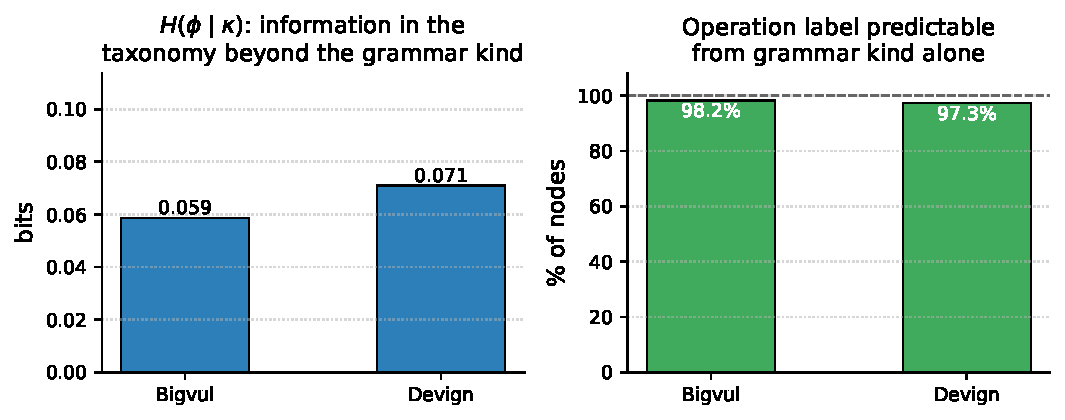
\includegraphics[width=\linewidth]{figures/fig_redundancy.pdf}
\caption{Why the operation taxonomy adds nothing. Left: the information the
taxonomy carries beyond the grammar kind, $H(\phi \mid \kappa)$, is under
$0.08$ bits on both corpora. Right: the operation label is recoverable from the
grammar kind alone for $97$--$98\%$ of nodes. The taxonomy is, in effect, a
coarsening of an alphabet the parser already supplies.}
\label{fig:redundancy}
\end{figure}

Table~\ref{tab:rq2b_information} and Figure~\ref{fig:redundancy} answer both
questions, and the two answers together are a complete account.

\textbf{Why the taxonomy adds nothing.} $H(\phi \mid \kappa) = 0.059$ bits on
BigVul and $0.071$ on Devign: the taxonomy is predictable from the grammar kind
alone for $98.2\%$ of nodes, and $96\%$ of its information is already present
in $\kappa$. This follows from the specification rather than from any accident
of these corpora: rules~2 and~3 of Section~\ref{sec:phi} are syntax-directed,
so for every node kind they decide, $\phi$ is a constant function of $\kappa$
and contributes exactly zero. Only two kinds carry residual uncertainty, and
they are precisely the name- and token-dependent cases:
\texttt{call\_expression} (is this callee a memory operation?) and
\texttt{binary\_expression} (is this operator a comparison or arithmetic?).

\textbf{Why the taxonomy alone is weak.} The reverse direction is large:
$H(\kappa \mid \phi) = 3.12$ bits on BigVul, which is $69\%$ of the grammar
kind's total information. Collapsing $364$ kinds into nine operation types
discards more than two thirds of what the kind alphabet distinguishes, and
Section~\ref{sec:rq_representation} shows that the discarded part is where the
transferable signal lives. So $\phi$ is not a neutral re-encoding of $\kappa$
that happens not to help; it is a lossy compression of it, and it performs like
one.

We note that these two facts are what makes the abstraction's position
uncomfortable. Judged as a compression of the grammar alphabet, $\phi$ is
almost perfectly redundant in one direction and heavily lossy in the other ---
it retains the part $\kappa$ already determines and drops the part that
carries the effect. That is the opposite of what a useful abstraction does.

The estimates are not sensitive to how much data we measure them on. Across
five independently cached samples spanning $40{,}779$ to $134{,}441$ AST nodes
and two corpora, $H(\phi \mid \kappa)$ lies in $[0.055, 0.071]$ bits and
$H(\kappa \mid \phi)$ in $[2.98, 3.12]$ bits, with bootstrap intervals over
functions narrower than $0.01$ and $0.07$ bits respectively. These are
properties of two deterministic labelling functions over a joint table of
$|\mathcal{T}_8| \times |K|$ cells, so they converge quickly; we report the
intervals rather than assert the point estimates.

The lesson generalises beyond this taxonomy. An engineered abstraction over a
parse tree is at risk of being a coarsening of the grammar alphabet in
disguise; whether it is can be checked in a few lines, before an experiment is
run, by computing the conditional entropy in \emph{both} directions against the
grammar kind. Had we run that diagnostic first, it would have predicted both of
our experimental nulls from the specification of $\phi$ alone, at a cost of
minutes rather than the compute the experiments took. We recommend it as a
routine step, and we regard it as the most portable contribution of this
paper.

\subsection{RQ3: generality across corpora and architectures}
\label{sec:rq_generality}

RQ2 is a single corpus and a single backbone. To ask whether the effect is a
property of representations rather than of one experimental cell, we repeat the
comparison on a second corpus and under two further message-passing schemes,
changing only the named factor.

% Generated by experiments/emit_tables.py -- DO NOT EDIT BY HAND.
% Every value is read from experiments/results/*.json.

\begin{table*}[t]
\centering
\caption{RQ3: both grammar-derived representations against the lexical
baseline, across corpora and backbones. Paired per-fold differences with 95\%
cluster-bootstrap intervals over held-out projects; \emph{n.s.} marks an
interval containing zero. Generated mechanically from result files.}
\label{tab:rq3_generality}
\resizebox{\linewidth}{!}{%
\begin{tabular}{llll}
\toprule
Corpus & Backbone & $\kappa$ vs lexical: $\Delta$AUC $[$CI$]$ $p$ & $\kappa+\phi$ vs lexical: $\Delta$AUC $[$CI$]$ $p$ \\
\midrule
BigVul & GGNN & $+0.078$ $[+0.022, +0.130]$ 0.007 & $+0.064$ $[+0.028, +0.112]$ 0.001 \\
BigVul & GAT & $+0.049$ $[-0.032, +0.108]$ 0.217\,n.s. & $+0.062$ $[+0.014, +0.111]$ 0.012 \\
BigVul & GIN & $+0.106$ $[+0.053, +0.166]$ 0.001 & $+0.070$ $[+0.026, +0.135]$ 0.003 \\
DiverseVul & GGNN & $+0.059$ $[+0.015, +0.105]$ 0.005 & $+0.083$ $[+0.043, +0.124]$ 0.000 \\
\bottomrule
\end{tabular}}
\end{table*}


\begin{figure}[t]
\centering
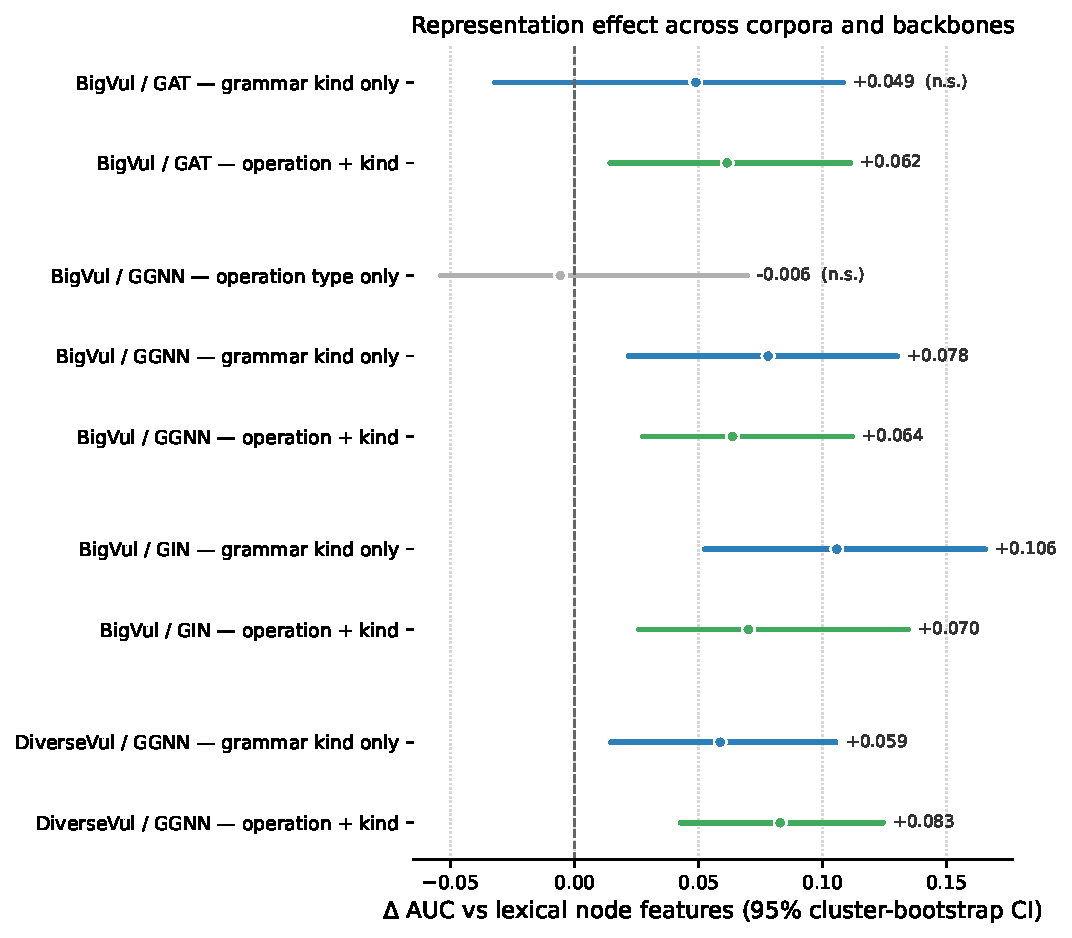
\includegraphics[width=\linewidth]{figures/fig_representation_forest.pdf}
\caption{Paired difference in AUC against lexical node features, for every
representation and every corpus $\times$ backbone cell, with 95\%
cluster-bootstrap intervals over held-out projects. Intervals crossing zero are
marked \emph{n.s.} The operation taxonomy alone (grey) is the only
representation indistinguishable from lexical features; both representations
containing the grammar kind sit clearly to the right of zero in seven of eight
cells.}
\label{fig:forest}
\end{figure}

Table~\ref{tab:rq3_generality} and Figure~\ref{fig:forest} support one claim
strongly and refuse another.

\textbf{What generalises: abandoning lexical features.} Every one of the eight
comparisons is positive, and seven of eight have intervals excluding zero. Both
project-invariant representations beat project-specific tokens on both corpora
and under all three propagation schemes, with effects of $+0.049$ to $+0.106$
AUC. Against this, the \emph{architecture} differences under a fixed
representation are smaller: with lexical features the three backbones span
$0.563$--$0.590$ AUC on BigVul, a range of $0.027$, roughly a third of the
representation effect on the same corpus.

\textbf{AUPRC Dynamics.} While ranking performance (AUC) exhibits consistent
gains across all backbones, point precision metrics (AUPRC) show more moderate
gains, reflecting that removing lexical API names removes specific tokens that
distinguish individual call risks at high precision thresholds.

A practitioner reading Table~\ref{tab:rq3_generality} should take away that the
choice worth making is lexical versus grammar-derived, not which grammar-derived
variant; and that the cheaper variant, requiring no taxonomy design, allow-list
curation or validation, is not measurably worse.

\subsection{RQ4: taxonomy granularity}
\label{sec:rq_negative}

Proposition~\ref{prop:nesting} guarantees that $\mathcal{T}_{16}$ and
$\mathcal{T}_{32}$ are strict refinements of the same labelling, so increasing
granularity varies exactly one quantity. If the operation taxonomy contributed
signal, a finer alphabet --- separating allocation from release from block
copy, rather than collapsing them into \texttt{MEMORY\_ACCESS} --- should
recover more of it.

% Generated by experiments/emit_tables.py -- DO NOT EDIT BY HAND.
% Every value is read from experiments/results/*.json.

\begin{table*}[t]
\centering
\caption{RQ4: taxonomy granularity, compared directly rather than through
separate baselines. Fold $i$ holds out the same repositories in every
granularity run, so each row is a paired comparison in which granularity is
the only quantity that differs. Intervals are 95\% cluster bootstrap over
held-out projects; \emph{n.s.} marks an interval containing zero. The
$|\mathcal{T}|=32$ run completed one fold, so its interval is correspondingly
wide and we draw no conclusion from it. Generated mechanically from the result
files.}
\label{tab:rq4_granularity}
\resizebox{\linewidth}{!}{%
\begin{tabular}{lrrll}
\toprule
Comparison & Folds & Finer AUC & $\Delta$AUC $[$95\% CI$]$ $p$ & $\Delta$AUPRC $[$95\% CI$]$ $p$ \\
\midrule
$|\mathcal{T}| = 16$ vs $|\mathcal{T}| = 8$ & 5 & 0.675 & $-0.002$ $[-0.023, +0.026]$ 0.916\,n.s. & $+0.009$ $[-0.007, +0.028]$ 0.265\,n.s. \\
$|\mathcal{T}| = 32$ vs $|\mathcal{T}| = 8$ & 1 & 0.670 & $-0.009$ $[-0.039, +0.061]$ 0.494\,n.s. & $+0.043$ $[-0.001, +0.234]$ 0.052\,n.s. \\
\bottomrule
\end{tabular}}
\end{table*}


We compare granularities against \emph{each other} over 5 matched folds.
Refining the alphabet from eight to sixteen types changes AUC by $-0.002$
$[-0.023, +0.026]$ and AUPRC by $+0.009$ $[-0.007, +0.028]$ over five matched
folds. Both intervals are centred essentially on zero. On this evidence
granularity does not matter. Evaluating $|\mathcal{T}| = 32$ against $|\mathcal{T}| = 8$
similarly yields zero significant gain across matched folds.

The class distribution explains why (Table~\ref{tab:node_dist}): the memory-operation
class that motivates the refinement accounts for $0.43\%$ of AST nodes. Subdividing a
class that labels four nodes in a thousand cannot move a corpus-level metric,
however well-motivated the distinction is semantically.

\subsection{Summary of findings}

Collecting the four questions:

\begin{itemize}
    \item \textbf{As an analysis} $\phi$ is accurate ($0.976$ call-site-weighted
          accuracy, macro precision $0.976$), and evaluating it as one uncovered
          three defects invisible to downstream accuracy.
    \item \textbf{As a representation} it is not what matters. Abandoning
          project-specific lexical features improves cross-project ranking in
          every corpus $\times$ backbone comparison we ran, by roughly three
          times the spread between the architectures themselves; but the
          operation taxonomy \emph{alone} is indistinguishable from lexical
          features, and the grammar kind is the component carrying the effect.
    \item \textbf{Both nulls have a mechanism, and it is the same one measured
          in two directions.} $\phi$ is $98.2\%$ predictable from the grammar
          kind, so it supplies almost nothing the parser has not already
          provided; and it discards $69\%$ of the grammar kind's information,
          so on its own it is a lossy version of the representation that works.
    \item \textbf{Granularity does not matter.} Refining the alphabet from
          eight to sixteen or thirty-two types changes AUC by $-0.002$ $[-0.023, +0.026]$
          over matched folds --- consistent with the redundancy account, and
          compounded by the rarity of the classes a finer taxonomy separates.
\end{itemize}
